%DO NOT MESS AROUND WITH THE CODE ON THIS PAGE UNLESS YOU %REALLY KNOW WHAT YOU ARE DOING
\chapter{Conclusion} \label{Conclusion}

\noindent This study presented a new Kinect-based gait recognition method that utilizes the 3D skeleton model in order to compute a robust representation of gait. It enables us to extract more complicated gait features from human walking sequences compared to conventional devices such as video cameras or wearable sensors. Although the set of 8 participants is statistically small, the maximum accuracy of 93.75\% obtained is promising and shows that reliable discrimination of individuals in an indoor ambiance is possible by this method. The following table summarizes the success rates obtained with different classification models.

\def\arraystretch{1.3}
\begin{table}[h]
\centering
\begin{tabular}{| p{3cm} | |p{3cm}|}
 \hline
\cellcolor{pink} Classifier & \cellcolor{pink} Accuracy \\ \hline
Linear SVM & 87.5 \% \\ \hline
Quadratic SVM & 93.75\% \\ \hline
Fine kNN & 81.24\% \\\hline
Complex Tree & 68.75\% \\ \hline
ANN & 93.75\% \\ \hline
\end{tabular}
\caption{ Different classifiers and their accuracy}
\end{table}

\newpage
\section{Future Work} \label{Future Work}
\noindent We are planning an extensive gait acquisition campaign to improve the validation of the classification results from a statistical viewpoint. The JRA (joint relative angle) data that we captured during a participants walk is not being used in this study. To provide a visual representation of the relevance of a particular JRA sequence in gait representation we constructed a heat map, where a high value corresponds to high relevance and low value corresponds to a low relevance. The heat map is symmetric on both side of the diagonal, since the JRA values between joints {J1, J2} and {J2, J1} are same.

\begin{figure}[h]
\centering
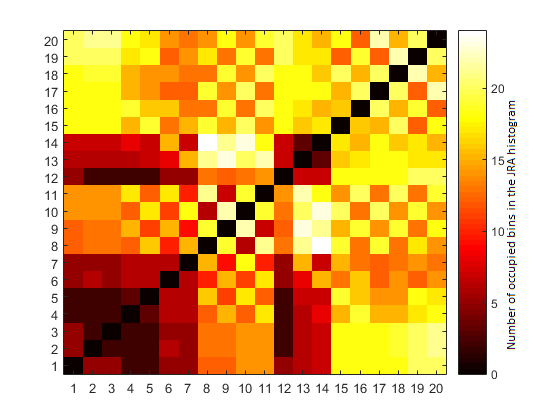
\includegraphics[scale=0.8]{heatMap.png}
\caption{Heat map of the 20x20 average matrix obtained for the average number of bins occupied for different JRA}
\end{figure}

\def\arraystretch{1.3}
\begin{table}[h]
\centering
\begin{tabular}{| p{3cm}| p{3cm}|p{3cm}| p{3cm}|}
 \hline
1 Head & 6 Elbow left & 11 Hand right & 16 Knee right  \\ \hline
2 Neck & 7 Elbow right & 12 Spine mid & 17 Ankle left  \\ \hline
3 Spine shoulder & 8 Wrist left & 13 Hip left & 18 Ankle right \\\hline
4 Shoulder left & 9 Wrist right & 14 Hip right & 19 Foot left \\ \hline
5 Shoulde right & 10 Hand left & 15 Knee left & 20 Foot right \\ \hline
\end{tabular}
\caption{ Body Joints}
\end{table}


\noindent We need to find a classifier or kernel that will take the collection of the most relevant JRA sequences from both the train and test samples as parameters and computes a similarity measure. This kernel will have to be robust against variable walking speed.
We could also investigate the possibility of using more than one Kinect sensor to track gait. From the applicative point of view we will consider other scenarios that go beyond classification, e.g. security and health/well-being contexts.
